\documentclass[12pt]{article}
\usepackage{bigints}
\usepackage{graphicx}			% Use this package to include images
\usepackage{amsmath}	
\usepackage{amssymb}
\usepackage{amsfonts}
\usepackage{polynom}
\usepackage{listings}
% A library of many standard math expressions
\graphicspath{ {./Images/} }
\usepackage[margin=1in]{geometry}% Sets 1in margins. 
\newcommand{\qed}[0]{$\blacksquare$}
\usepackage{fancyhdr}			% Creates headers and footers
\usepackage{enumerate}          %These two package give custom labels to a list
\usepackage[shortlabels]{enumitem}


% Creates the header and footer. You can adjust the look and feel of these here.
\pagestyle{fancy}
\fancyhead[l]{Aditya Gupta}
\fancyhead[c]{Math 135 Homework \#3}
\fancyhead[r]{\today}
\fancyfoot[c]{\thepage}
\renewcommand{\headrulewidth}{0.2pt} %Creates a horizontal line underneath the header
\setlength{\headheight}{15pt} %Sets enough space for the header
\begin{document}
\begin{enumerate}
\item [50. ]
\[
f'(x) = -2f(x)
\]

This can be solved by separating variables:
\[
\frac{f'(x)}{f(x)} = -2
\]
    
Integrating both sides:
\[
\ln|f(x)| = -2x + C
\]

Exponentiating both sides:
\[
f(x) = e^C e^{-2x} = Ce^{-2x}
\]

Using the initial condition \( f(0) = 1 \):
\[
f(0) = Ce^{0} = C \implies C = 1
\]

Thus, the solution is:
\[
f(x) = e^{-2x}
\]

To express \( f(x) \) as a power series:
\[
f(x) = e^{-2x} = \sum_{n=0}^\infty \frac{(-2x)^n}{n!}
\]

Simplify the general term:
\[
f(x) = \sum_{n=0}^\infty \frac{(-2)^n x^n}{n!}
\]

The sum of the series is the value of \( f(x) \) at \( x = 1 \):
\[
\text{Sum of the series} = f(1) = e^{-2}
\]

Final answer:
\[
f(x) = \sum_{n=0}^\infty \frac{(-2)^n x^n}{n!}, \quad \text{Sum of the series} = e^{-2}
\]

\item [2. ]
\[
\sum_{k=0}^\infty \frac{\sin k}{2^k}
\]

We know that:
\[
\sin k = \text{Im}(e^{ik}),
\]
so the series can be rewritten as:
\[
\sum_{k=0}^\infty \frac{\sin k}{2^k} = \text{Im}\left( \sum_{k=0}^\infty \frac{e^{ik}}{2^k} \right).
\]

The term \(\frac{e^{ik}}{2^k}\) forms a geometric series with common ratio \(r = \frac{e^i}{2}\), and since \(|r| = \frac{1}{2} < 1\), the series converges. The sum of the geometric series is given by:
\[
\sum_{k=0}^\infty r^k = \frac{1}{1 - r}.
\]

Substituting \(r = \frac{e^i}{2}\):
\[
\sum_{k=0}^\infty \frac{e^{ik}}{2^k} = \frac{1}{1 - \frac{e^i}{2}}.
\]

Simplify \(1 - \frac{e^i}{2}\):
\[
1 - \frac{e^i}{2} = 1 - \frac{\cos 1 + i \sin 1}{2} = \frac{2 - (\cos 1 + i \sin 1)}{2}.
\]

Thus:
\[
\frac{1}{1 - \frac{e^i}{2}} = \frac{2}{2 - (\cos 1 + i \sin 1)}.
\]

Let \(A = 2 - \cos 1\) and \(B = \sin 1\). Then:
\[
\frac{2}{2 - (\cos 1 + i \sin 1)} = \frac{2}{A + iB}.
\]

To separate the imaginary part, multiply numerator and denominator by the conjugate of the denominator:
\[
\frac{2}{A + iB} = \frac{2(A - iB)}{A^2 + B^2}.
\]

The imaginary part is:
\[
\text{Im}\left(\frac{2}{A + iB}\right) = \frac{2B}{A^2 + B^2}.
\]

Substitute back \(A = 2 - \cos 1\) and \(B = \sin 1\):
\[
\text{Im}\left(\frac{2}{2 - (\cos 1 + i \sin 1)}\right) = \frac{2 \sin 1}{(2 - \cos 1)^2 + (\sin 1)^2}.
\]

Numerically, this evaluates to:
\[
\sum_{k=0}^\infty \frac{\sin k}{2^k} \approx 0.5928.
\]

I used the geometric series test for this

\item [3. ]
We prove by induction on \( k \geq 0 \) that:

\[
\frac{1}{(1-x)^{k+1}} = \sum_{n=0}^\infty \binom{n+k}{k} x^n, \quad \text{for } |x| < 1.
\]

Base Case: For \( k = 0 \), the left-hand side becomes:

\[
\frac{1}{(1-x)^{0+1}} = \frac{1}{1-x}.
\]

The right-hand side becomes:

\[
\sum_{n=0}^\infty \binom{n+0}{0} x^n = \sum_{n=0}^\infty x^n.
\]

The geometric series \( \sum_{n=0}^\infty x^n \) converges to \( \frac{1}{1-x} \) for \( |x| < 1 \).

Thus, the base case holds.

Inductive Step: Assume the formula holds for \( k = m \), i.e.,

\[
\frac{1}{(1-x)^{m+1}} = \sum_{n=0}^\infty \binom{n+m}{m} x^n.
\]

We need to prove it for \( k = m+1 \), i.e.,

\[
\frac{1}{(1-x)^{m+2}} = \sum_{n=0}^\infty \binom{n+(m+1)}{m+1} x^n.
\]

The left-hand side for \( k = m+1 \) is:

\[
\frac{1}{(1-x)^{m+2}} = \frac{d}{dx} \left( \frac{1}{(1-x)^{m+1}} \right).
\]

Using the inductive hypothesis:

\[
\frac{1}{(1-x)^{m+1}} = \sum_{n=0}^\infty \binom{n+m}{m} x^n.
\]

Take the derivative of both sides:

\[
\frac{d}{dx} \left( \frac{1}{(1-x)^{m+1}} \right) = \frac{d}{dx} \left( \sum_{n=0}^\infty \binom{n+m}{m} x^n \right).
\]

On the left-hand side:

\[
\frac{d}{dx} \left( \frac{1}{(1-x)^{m+1}} \right) = (m+1) \cdot \frac{1}{(1-x)^{m+2}}.
\]

On the right-hand side, differentiate term by term:

\[
\frac{d}{dx} \left( \sum_{n=0}^\infty \binom{n+m}{m} x^n \right) = \sum_{n=1}^\infty \binom{n+m}{m} n x^{n-1}.
\]

Reindex the sum by letting \( n' = n-1 \) (so \( n = n'+1 \)):

\[
\sum_{n=1}^\infty \binom{n+m}{m} n x^{n-1} = \sum_{n'=0}^\infty \binom{(n'+1)+m}{m} (n'+1) x^{n'}.
\]

Simplify the binomial coefficient:

\[
\binom{(n'+1)+m}{m} = \binom{n'+m+1}{m}.
\]

Thus, the sum becomes:

\[
\sum_{n'=0}^\infty \binom{n'+m+1}{m+1} x^{n'}.
\]

Relabel \( n' \to n \) for clarity:

\[
\sum_{n=0}^\infty \binom{n+m+1}{m+1} x^n.
\]

This matches the right-hand side for \( k = m+1 \):

\[
\frac{1}{(1-x)^{m+2}} = \sum_{n=0}^\infty \binom{n+(m+1)}{m+1} x^n.
\]

Thus, by induction, the formula holds for all \( k \geq 0 \).

\item [4. ]
We solve \( z^4 + z^2 + 1 = 0 \).

Let \( w = z^2 \). Then \( z^4 = w^2 \), and the equation becomes:

\[
w^2 + w + 1 = 0.
\]

The quadratic equation \( w^2 + w + 1 = 0 \) can be solved using the quadratic formula:

\[
w = \frac{-b \pm \sqrt{b^2 - 4ac}}{2a}.
\]

Here, \( a = 1 \), \( b = 1 \), \( c = 1 \). Substituting these values:

\[
w = \frac{-1 \pm \sqrt{1^2 - 4(1)(1)}}{2(1)} = \frac{-1 \pm \sqrt{-3}}{2}.
\]

Since \( \sqrt{-3} = i\sqrt{3} \), we have:

\[
w = \frac{-1 \pm i\sqrt{3}}{2}.
\]

Let:

\[
w_1 = \frac{-1 + i\sqrt{3}}{2}, \quad w_2 = \frac{-1 - i\sqrt{3}}{2}.
\]

Now, we solve \( z^2 = w_1 \) and \( z^2 = w_2 \).

For \( z^2 = w_1 = \frac{-1 + i\sqrt{3}}{2} \), we find \( z \) using the formula for the square root of a complex number:

\[
\sqrt{a + bi} = \pm \left( \sqrt{\frac{|a+bi| + a}{2}} + i \cdot \text{sgn}(b) \sqrt{\frac{|a+bi| - a}{2}} \right),
\]

where \( |a+bi| = \sqrt{a^2 + b^2} \).

Here, \( a = -\frac{1}{2} \) and \( b = \frac{\sqrt{3}}{2} \). First, calculate the modulus:

\[
\left| \frac{-1 + i\sqrt{3}}{2} \right| = \sqrt{\left(-\frac{1}{2}\right)^2 + \left(\frac{\sqrt{3}}{2}\right)^2} = \sqrt{\frac{1}{4} + \frac{3}{4}} = \sqrt{1} = 1.
\]

The formula becomes:

\[
\sqrt{\frac{-1 + i\sqrt{3}}{2}} = \pm \left( \sqrt{\frac{1 + \left(-\frac{1}{2}\right)}{2}} + i \sqrt{\frac{1 - \left(-\frac{1}{2}\right)}{2}} \right).
\]

Simplify:

\[
\sqrt{\frac{-1 + i\sqrt{3}}{2}} = \pm \left( \sqrt{\frac{1 - 1/2}{2}} + i \sqrt{\frac{1 + 1/2}{2}} \right).
\]

\[
\sqrt{\frac{-1 + i\sqrt{3}}{2}} = \pm \left( \sqrt{\frac{1}{4}} + i \sqrt{\frac{3}{4}} \right).
\]

\[
\sqrt{\frac{-1 + i\sqrt{3}}{2}} = \pm \left(\frac{1}{2} + i\frac{\sqrt{3}}{2}\right).
\]

Thus, the two roots for this case are:

\[
z = \frac{1}{2} + i\frac{\sqrt{3}}{2}, \quad z = -\frac{1}{2} - i\frac{\sqrt{3}}{2}.
\]

For \( z^2 = w_2 = \frac{-1 - i\sqrt{3}}{2} \), repeat the process:

\[
\sqrt{\frac{-1 - i\sqrt{3}}{2}} = \pm \left( \sqrt{\frac{1 + \left(-\frac{1}{2}\right)}{2}} + i \cdot \text{sgn}\left(-\frac{\sqrt{3}}{2}\right) \sqrt{\frac{1 - \left(-\frac{1}{2}\right)}{2}} \right).
\]

Simplify:

\[
\sqrt{\frac{-1 - i\sqrt{3}}{2}} = \pm \left( \sqrt{\frac{1 - 1/2}{2}} - i \sqrt{\frac{1 + 1/2}{2}} \right).
\]

\[
\sqrt{\frac{-1 - i\sqrt{3}}{2}} = \pm \left(\frac{1}{2} - i\frac{\sqrt{3}}{2}\right).
\]

Thus, the two roots for this case are:

\[
z = \frac{1}{2} - i\frac{\sqrt{3}}{2}, \quad z = -\frac{1}{2} + i\frac{\sqrt{3}}{2}.
\]

The four roots of the equation are:

\[
z = \frac{1}{2} + i\frac{\sqrt{3}}{2}, \quad z = -\frac{1}{2} - i\frac{\sqrt{3}}{2}, \quad z = \frac{1}{2} - i\frac{\sqrt{3}}{2}, \quad z = -\frac{1}{2} + i\frac{\sqrt{3}}{2}.
\]
\newpage
\item [5. ]
\begin{enumerate}
    \item Below is the geometric representation of the sum of 2 complex numbers 
    
    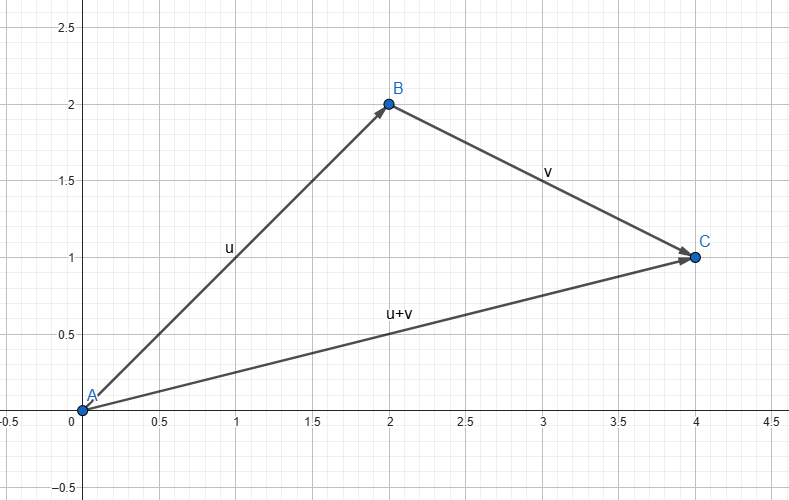
\includegraphics[width=0.75\linewidth]{Math 135//Assignments/image.png}

    Let \( z_1 = a_1 + i a_2 \) and \( z_2 = b_1 + i b_2 \), where \( a_1, a_2, b_1, b_2 \in \mathbb{R} \).

Start by noting that the square of any real number is always non-negative:

\[
0 \leq (a_1b_2 - a_2b_1)^2
\]

Expand the square on the right-hand side:

\[
(a_1b_2 - a_2b_1)^2 = a_1^2b_2^2 - 2a_1a_2b_1b_2 + a_2^2b_1^2
\]

Rearrange terms to isolate the cross-product term:

\[
a_1^2b_2^2 + a_2^2b_1^2 \geq 2a_1a_2b_1b_2
\]

Now add \( a_1^2b_1^2 + a_2^2b_2^2 \) to both sides to form a complete expansion:

\[
a_1^2b_1^2 + a_1^2b_2^2 + a_2^2b_1^2 + a_2^2b_2^2 \geq a_1^2b_1^2 + a_2^2b_2^2 + 2a_1a_2b_1b_2
\]

Factor both sides of the inequality:

\[
(a_1^2 + a_2^2)(b_1^2 + b_2^2) \geq (a_1b_1 + a_2b_2)^2
\]

Take the square root of both sides:

\[
\sqrt{(a_1^2 + a_2^2)(b_1^2 + b_2^2)} \geq |a_1b_1 + a_2b_2|
\]

Express this in terms of the modulus of \( z_1 \) and \( z_2 \), noting that \( |z_1|^2 = a_1^2 + a_2^2 \) and \( |z_2|^2 = b_1^2 + b_2^2 \):

\[
|z_1|^2 + 2|z_1||z_2| + |z_2|^2 \geq |z_1 + z_2|^2
\]

Take the square root again to arrive at the desired inequality:

\[
|z_1| + |z_2| \geq |z_1 + z_2|
\]

Thus, we have proven the triangle inequality:

\[
|z_1 + z_2| \leq |z_1| + |z_2|
\]

\item 
We aim to prove that:
\[
|z_1 + z_2|^2 + |z_1 - z_2|^2 = 2(|z_1|^2 + |z_2|^2).
\]

Let \( z_1 = a_1 + i a_2 \) and \( z_2 = b_1 + i b_2 \), where \( a_1, a_2, b_1, b_2 \in \mathbb{R} \). First, expand \( |z_1 + z_2|^2 \) and \( |z_1 - z_2|^2 \).

\[
|z_1 + z_2|^2 = (a_1 + b_1)^2 + (a_2 + b_2)^2
\]

\[
= a_1^2 + 2a_1b_1 + b_1^2 + a_2^2 + 2a_2b_2 + b_2^2
\]

\[
= a_1^2 + a_2^2 + b_1^2 + b_2^2 + 2(a_1b_1 + a_2b_2)
\]

Now expand \( |z_1 - z_2|^2 \):

\[
|z_1 - z_2|^2 = (a_1 - b_1)^2 + (a_2 - b_2)^2
\]

\[
= a_1^2 - 2a_1b_1 + b_1^2 + a_2^2 - 2a_2b_2 + b_2^2
\]

\[
= a_1^2 + a_2^2 + b_1^2 + b_2^2 - 2(a_1b_1 + a_2b_2)
\]

Add the two expressions for \( |z_1 + z_2|^2 \) and \( |z_1 - z_2|^2 \):

\[
|z_1 + z_2|^2 + |z_1 - z_2|^2 = \big(a_1^2 + a_2^2 + b_1^2 + b_2^2 + 2(a_1b_1 + a_2b_2)\big) + \big(a_1^2 + a_2^2 + b_1^2 + b_2^2 - 2(a_1b_1 + a_2b_2)\big)
\]

Simplify the terms:

\[
|z_1 + z_2|^2 + |z_1 - z_2|^2 = 2(a_1^2 + a_2^2 + b_1^2 + b_2^2)
\]

Recognize that \( a_1^2 + a_2^2 = |z_1|^2 \) and \( b_1^2 + b_2^2 = |z_2|^2 \):

\[
|z_1 + z_2|^2 + |z_1 - z_2|^2 = 2(|z_1|^2 + |z_2|^2)
\]
    
\end{enumerate}

\end{enumerate}




\end{document}
